\documentclass[aspectratio=169, 11pt, t]{beamer}
\usepackage{beamerthemesloan}
\usepackage{appendixnumberbeamer}
\graphicspath{{figures/}}

\title{Prediction Markets as Macro Data}
\subtitle{Kalshi vs.\ fed funds futures}
\question{Are Kalshi's prices on FOMC decisions good forecasts, and how do they compare with fed funds futures?}
% TODO: check names and order
\author{Andres Blanco Prada \\ Panos Koutsoukos \\ Connor Rippert \\ Vish}
\date{Progress update \textbar\ October 2026}

\begin{document}

{\setbeamertemplate{headline}{}\setbeamertemplate{footline}{}
\begin{frame}[noframenumbering]
  \titlepage
\end{frame}}

% =========================================================================
\section{Replication}
% =========================================================================
\begin{frame}{We replicate Diercks--Katz--Wright and improve on it}
  \framesubtitle{Kalshi-implied policy rate vs.\ the rate actually set, 41 FOMC meetings 2021--2026}
  \source{kalshi\_fed/}
  \begin{columns}[T]
    \begin{column}{0.68\textwidth}
      \begin{tikzpicture}
        \begin{axis}[sloan, width=\linewidth, height=5.6cm,
            xmin=0, xmax=162, ymin=0, ymax=56, xtick={1,30,60,90,120,160},
            xlabel={Days before the meeting}, ylabel={Mean abs.\ error (bp)},
            legend pos=north west]
          \addplot[benchline, no marks] table[x=h, y=dkw] {data/dkw_mae_curve.dat};
          \addlegendentry{DKW method (last trades)}
          \addplot[kalshiline, no marks] table[x=h, y=ours] {data/dkw_mae_curve.dat};
          \addlegendentry{Our method (quotes)}
        \end{axis}
      \end{tikzpicture}
    \end{column}
    \begin{column}{0.28\textwidth}
      \vspace{6pt}
      \keyfig{41/41}{meetings called correctly the day before}
      \keyfig{$-$14\%}{average error over 1--160 days (17.9 vs.\ 20.8bp)}
      {\footnotesize\color{sloangray}Why: 40--45\% of last trades are over a week old.\par}
    \end{column}
  \end{columns}
\end{frame}

% =========================================================================
\section{Calibration}
% =========================================================================
\begin{frame}{Fed-decision prices show a favorite--longshot pattern}
  \framesubtitle{Share of contracts that paid out, by price, 1--21 days before the meeting}
  \source{02\_calibration\_kalshi.py}
  \begin{columns}[T]
    \begin{column}{0.6\textwidth}
      \centering
      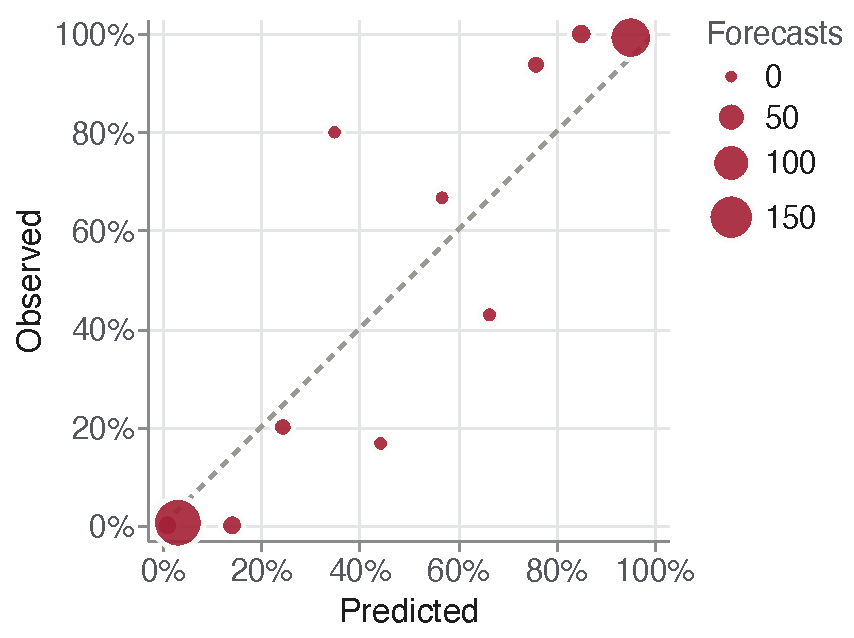
\includegraphics[height=5.6cm]{reliability_fed}
    \end{column}
    \begin{column}{0.36\textwidth}
      \vspace{10pt}
      \keyfig{0.5\%}{payout rate of contracts priced 1--10\textcent{} (avg.\ price 3.1\textcent)}
      \keyfig{99.3\%}{payout rate of contracts priced 90--99\textcent{} (avg.\ 95.3\textcent)}
      {\footnotesize\color{sloangray}Bubble size = forecasts. 632 forecasts, 28 meetings. Middle bins hold 2--6 meetings each.\par}
    \end{column}
  \end{columns}
\end{frame}

\begin{frame}{A calibration regression confirms the pattern}
  \framesubtitle{$P(\text{YES}) = \Lambda(\alpha + \beta\,\operatorname{logit} p)$; calibrated means $\alpha = 0$, $\beta = 1$}
  \source{02\_calibration\_kalshi.py}
  \begin{columns}[T]
    \begin{column}{0.6\textwidth}
      \centering
      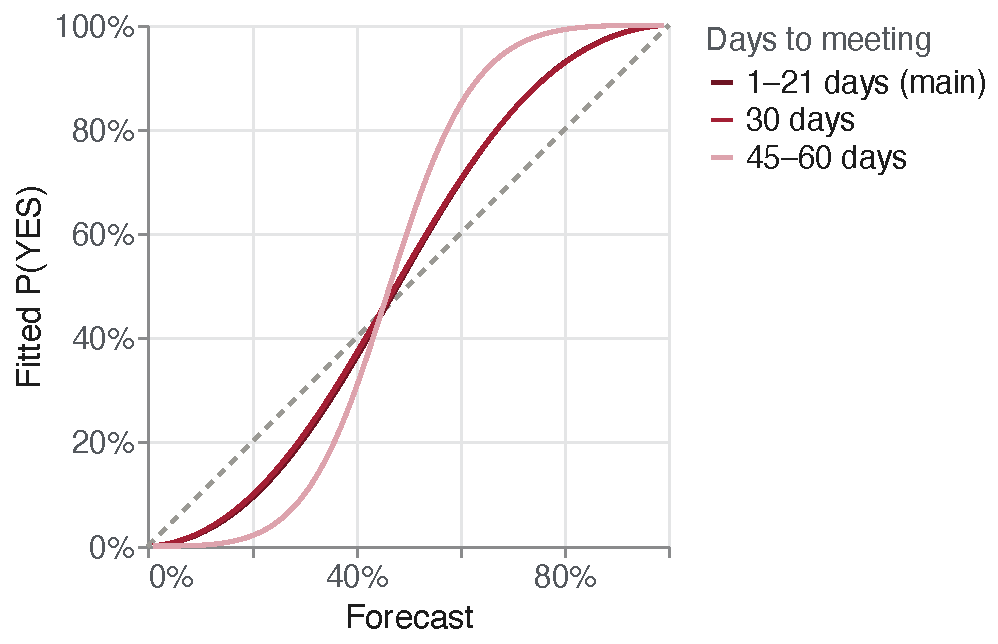
\includegraphics[height=5.6cm]{fitted_by_horizon}
    \end{column}
    \begin{column}{0.36\textwidth}
      \vspace{10pt}
      \keyfig{1.75}{calibration slope $\beta$ at 1--21 days (SE 0.45; bootstrap 95\% CI 1.22--3.54)}
      \keyfig{p = 0.01}{joint test of calibration (cluster bootstrap)}
      {\footnotesize\color{sloangray}$\beta > 1$: favorites win more than priced, longshots less. Errors clustered by meeting (28). No significant change after the May 2025 liquidity jump.\par}
    \end{column}
  \end{columns}
\end{frame}

% =========================================================================
\section{Fed funds futures}
% =========================================================================
\begin{frame}{Futures give a benchmark probability for every meeting}
  \framesubtitle{The WIRP-style method: from futures prices to outcome probabilities}
  \source{03\_fedfunds\_vs\_kalshi.py}
  \vspace{4pt}
  \centering
  \begin{tikzpicture}[
      flowbox/.style={draw=rule, fill=white, line width=0.6pt, align=center, font=\footnotesize,
        text width=2.75cm, minimum height=1.45cm, inner sep=4pt},
      arr/.style={-{Stealth[length=5pt]}, sloanred, line width=1pt}]
    \node[flowbox] (a) {\textbf{Futures price}\\[1pt]{\scriptsize FF1--FF13, daily}};
    \node[flowbox, right=0.55cm of a] (b) {\textbf{Avg.\ rate per month}\\[1pt]{\scriptsize $100 - P$}};
    \node[flowbox, right=0.55cm of b] (c) {\textbf{Rate after meeting}\\[1pt]{\scriptsize un-blend the meeting month}};
    \node[flowbox, right=0.55cm of c, draw=sloanred, fill=wash] (d) {\textbf{Expected move $x$}\\[1pt]{\scriptsize in 25bp steps}};
    \draw[arr] (a) -- (b); \draw[arr] (b) -- (c); \draw[arr] (c) -- (d);
  \end{tikzpicture}

  \vspace{8pt}
  \begin{columns}[T]
    \begin{column}{0.5\textwidth}
      \centering
      \begin{tikzpicture}
        \begin{axis}[sloan, width=6.6cm, height=3.7cm, ybar, sloanbars, bar width=14pt, ymin=0, ymax=1.12,
            symbolic x coords={Cut 50+, Cut 25, Hold, Hike 25, Hike 50+}, xtick=data,
            ytick={0,0.5,1}, ylabel={Probability},
            nodes near coords, nodes near coords style={font=\scriptsize, color=ink,
              /pgf/number format/.cd, fixed, precision=2}]
          \addplot[fill=bench, draw=none] coordinates
            {(Cut 50+,0.088) (Cut 25,0.912) (Hold,0) (Hike 25,0) (Hike 50+,0)};
        \end{axis}
      \end{tikzpicture}
    \end{column}
    \begin{column}{0.42\textwidth}
      \vspace{6pt}
      {\footnotesize\textbf{Example:} 30 Jul 2024, for the 18 Sep meeting.\\
      $x = -1.09$ steps $\Rightarrow$ 91\% cut 25bp, 9\% cut 50bp.\par\vspace{6pt}
      \color{sloangray}All mass sits on the two outcomes next to $x$, so the futures can never price the tails.\par}
    \end{column}
  \end{columns}
\end{frame}

% =========================================================================
\section{Kalshi vs.\ futures}
% =========================================================================
\begin{frame}{Kalshi is calibrated like futures and slightly more accurate}
  \framesubtitle{Hold and $\pm$25bp outcomes, both read at 15:00 ET and scored against the decision}
  \source{03\_fedfunds\_vs\_kalshi.py}
  \begin{columns}[T]
    \begin{column}{0.6\textwidth}
      \centering
      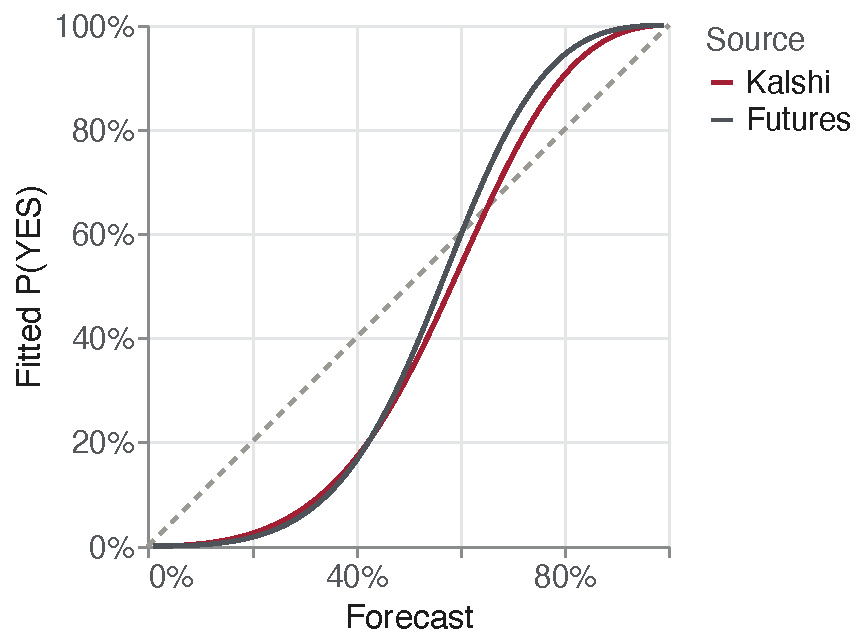
\includegraphics[height=5.6cm]{ff_vs_kalshi_fitted}
    \end{column}
    \begin{column}{0.36\textwidth}
      \vspace{10pt}
      \keyfig{2.14 vs.\ 2.48}{calibration slope $\beta$, Kalshi vs.\ futures (1--21 days): both under-confident}
      \keyfig{0.039 vs.\ 0.046}{Brier score at 30 days, Kalshi vs.\ futures}
      {\footnotesize\color{sloangray}Kalshi scores better at 1--30 days, futures at 45--60 days (few meetings). Kalshi prices moves beyond 25bp higher.\par}
    \end{column}
  \end{columns}
\end{frame}

% =========================================================================
\section{Lead--lag}
% =========================================================================
\begin{frame}{Intraday, futures lead Kalshi by about five minutes}
  \framesubtitle{Correlation of 5-minute changes in the expected move, Mar--Oct 2026, 5 meetings}
  \source{04\_leadlag\_fedfunds\_kalshi.py}
  \begin{columns}[T]
    \begin{column}{0.64\textwidth}
      \centering
      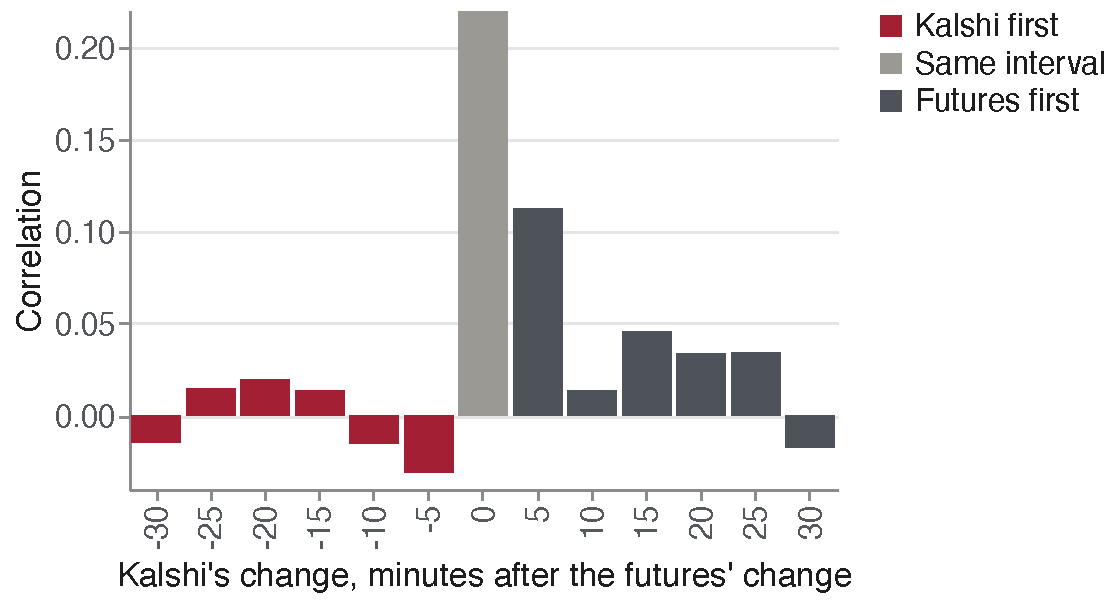
\includegraphics[width=\linewidth]{leadlag_xcorr}
    \end{column}
    \begin{column}{0.32\textwidth}
      \vspace{4pt}
      \keyfig{0.22}{same 5 minutes: most co-movement is simultaneous}
      \keyfig{p $<$ 0.001}{past futures moves predict Kalshi (Granger; p = 0.06 the other way)}
      \keyfig{16\%}{of a large futures move shows up in Kalshi within 15 minutes}
    \end{column}
  \end{columns}
\end{frame}

% =========================================================================
% Appendix
% =========================================================================
\sloanappendix
\dividerframe{Appendix}

\section{Plan}
\begin{frame}{Research questions and next steps}
  \begin{columns}[T]
    \begin{column}{0.47\textwidth}
      {\color{sloanred}\bfseries\small Questions}\par\vspace{4pt}
      \begin{itemize}\footnotesize
        \item \textbf{RQ1 Calibration.} Are Kalshi prices rational forecasts? Favorite--longshot bias? Better than futures and surveys? \emph{First results in.}
        \item \textbf{RQ2 Price discovery.} How fast do prices absorb CPI, payrolls and FOMC news vs.\ futures? \emph{Lead--lag started.}
        \item \textbf{RQ3 Forecasting.} Use Kalshi distributions to predict CPI, unemployment and GDP. \emph{Not started.}
      \end{itemize}
    \end{column}
    \begin{column}{0.47\textwidth}
      {\color{sloanred}\bfseries\small Next steps}\par\vspace{4pt}
      \begin{itemize}\footnotesize
        \item Lead--lag around FOMC statements (14:00 ET) vs.\ quiet times; extend the intraday futures sample before March 2026.
        \item Information shares (Hasbrouck) next to the Granger tests.
        \item Formal Kalshi vs.\ futures score test (e.g.\ Diebold--Mariano).
        \item Rerun the daily futures comparison on refreshed candles (meetings after Sep 2025).
        \item Add SPF and Bloomberg consensus benchmarks for CPI and payrolls.
      \end{itemize}
    \end{column}
  \end{columns}
\end{frame}

\section{Data}
\begin{frame}{Dataset: every Kalshi trade and 1-minute quote}
  \source{00\_fetch\_data\_kalshi.py}
  \centering\footnotesize
  \begin{tabular}{lrrrrl}
    \toprule
    Series & Events & Contracts & Trades & Volume & Since \\
    \midrule
    Fed decision (KXFEDDECISION) & 40 & 200 & 770,571 & 620M & Apr 2023 \\
    CPI m/m (KXCPI) & 67 & 552 & 204,598 & 25.5M & Jul 2021 \\
    Core CPI m/m (KXCPICORE) & 56 & 500 & 33,259 & 7.7M & Jul 2022 \\
    CPI y/y (KXCPIYOY) & 49 & 713 & 241,413 & 37.9M & Dec 2022 \\
    Payrolls (KXPAYROLLS) & 45 & 422 & 116,507 & 19.6M & Mar 2023 \\
    \midrule
    Fed funds ladders (KXFED) & 52 & 660 & $\sim$222,000 & 59M & Jul 2021 \\
    \bottomrule
  \end{tabular}

  \vspace{10pt}
  \raggedright
  \begin{itemize}\footnotesize
    \item 10.4M one-minute candles. 100\% of 2,155 settled contracts match Kalshi's reported volume within $\pm$1\%.
    \item Futures: Bloomberg FF1--FF13, EFFR and target range, daily 2000--2026; 1-minute bid/ask bars Mar--Oct 2026.
    \item Fed outcomes: 19 holds, 5 cuts of 25bp, 1 cut of 50bp (Sep 2024), 3 hikes of 25bp.
  \end{itemize}
\end{frame}

\begin{frame}{Kalshi has become a deep market for Fed decisions}
  \framesubtitle{Contracts traded per month, all KXFEDDECISION meetings (log scale)}
  \source{01\_eda\_kalshi.py}
  \centering
  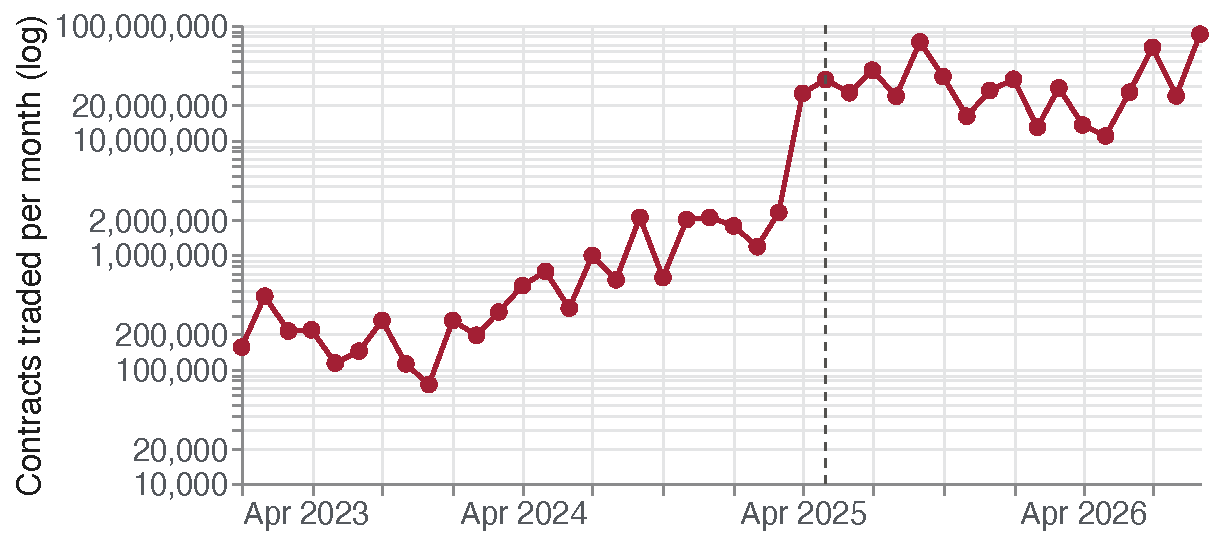
\includegraphics[width=0.85\linewidth]{monthly_volume}

  {\footnotesize\color{sloangray}620M contracts since 2023; volume rose about 10$\times$ in spring 2025. Median bid--ask spread 1\textcent.\par}
\end{frame}

\begin{frame}{Literature: what is known and what we add}
  \centering\footnotesize
  \renewcommand{\arraystretch}{1.25}
  \begin{tabular}{>{\raggedright\arraybackslash}p{3.5cm}>{\raggedright\arraybackslash}p{5.5cm}>{\raggedright\arraybackslash}p{4.2cm}}
    \toprule
    Paper & Finding & Gap we target \\
    \midrule
    Diercks, Katz \& Wright (2026) & Kalshi distributions for fed funds, CPI, GDP; CPI beats Bloomberg consensus & No Brier/log scores, no bias test, daily only \\
    B\"urgi, Deng \& Whelan (2026) & Strong favorite--longshot bias overall; weak in economics contracts & Test on macro with clean specification \\
    Bartlett \& O'Hara (2026) & Microstructure of 41.6M Kalshi trades & No forecast evaluation \\
    Wolfers \& Zitzewitz (2004) & Contract design reveals mean, median, distribution & Early evidence: 16 obs.\ \\
    Kelly et al.\ (2026) & Transformer stochastic discount factor & Only regularized ideas fit our sample (RQ3) \\
    \bottomrule
  \end{tabular}
\end{frame}

\section{Replication}
\begin{frame}{Kalshi-implied rate paths vs.\ the realized target}
  \framesubtitle{Each line: the path the market implied on one date; red steps: the actual upper bound}
  \source{kalshi\_fed/}
  \centering
  \begin{tikzpicture}
    \begin{axis}[sloan, width=13cm, height=5.6cm, xmin=2021.5, xmax=2027.3,
        ymin=0, ymax=6, xtick={2022,2023,2024,2025,2026,2027},
        xticklabel style={/pgf/number format/1000 sep={}},
        ylabel={Upper bound (\%)}, unbounded coords=jump]
      \addplot[benchline, solid, line width=0.6pt, opacity=0.6, no marks] table[x=x, y=rate] {data/hairs.dat};
      \addplot[kalshiline, const plot, no marks] table[x=x, y=upper_bound] {data/realized_target.dat};
    \end{axis}
  \end{tikzpicture}
\end{frame}

\begin{frame}{Replication accuracy by horizon}
  \source{kalshi\_fed/data/validation.json}
  \begin{columns}[T]
    \begin{column}{0.6\textwidth}
      \begin{tikzpicture}
        \begin{axis}[sloan, width=\linewidth, height=5.5cm, ybar, sloanbars, bar width=10pt, ymin=0, ymax=25,
            xtick=data, xticklabels from table={data/dkw_horizon_bars.dat}{horizon},
            ylabel={Mean abs.\ error (bp)}, legend pos=north west]
          \addplot[fill=bench, draw=none] table[x=i, y=dkw] {data/dkw_horizon_bars.dat};
          \addlegendentry{DKW}
          \addplot[fill=sloanred, draw=none] table[x=i, y=ours] {data/dkw_horizon_bars.dat};
          \addlegendentry{Ours}
        \end{axis}
      \end{tikzpicture}
    \end{column}
    \begin{column}{0.36\textwidth}
      \footnotesize
      \textbf{vs.\ NY Fed dealer survey}\\[2pt]
      132 forecasts, 37 meetings:\\
      survey 19.1bp, Kalshi mode 17.0bp.\par\vspace{8pt}
      \textbf{Method}\\[2pt]
      Mid quote if spread $\le$ 20\textcent, else last trade (20--40\textcent) or dropped; weighted isotonic fit across strikes.\par\vspace{8pt}
      \textbf{On DKW's 2022--25 window}\\[2pt]
      19.9 vs.\ 22.7bp (1--160 days).
    \end{column}
  \end{columns}
\end{frame}

\section{Calibration}
\begin{frame}{Calibration regression: estimates}
  \framesubtitle{Logit of outcome on logit of price; meeting-clustered SEs; 999-draw cluster bootstrap}
  \source{02\_calibration\_kalshi.py}
  \centering\scriptsize
  \setlength{\tabcolsep}{4pt}
  \begin{tabular}{lrrrrrr}
    \toprule
    Horizon & Obs.\ / meetings & $\alpha$ (SE) & $\beta$ (SE) & $\beta$ 95\% CI (boot) & p($\beta$=1) & p joint (boot) \\
    \midrule
    1--21 days (main) & 454 / 28 & 0.141 (0.030) & 1.751 (0.453) & [1.22, 3.54] & 0.097 & 0.010 \\
    30 days & 78 / 27 & 0.165 (0.062) & 1.723 (0.533) & [1.11, 2.77] & 0.175 & 0.008 \\
    45--60 days & 100 / 18 & 0.445 (0.186) & 3.133 (1.058) & [1.97, 13.66] & 0.044 & 0.189 \\
    \bottomrule
  \end{tabular}

  \vspace{12pt}
  \raggedright
  \begin{itemize}\footnotesize
    \item $\beta > 1$ at every horizon: under-confident prices, the favorite--longshot pattern.
    \item $\alpha > 0$ is significant: the YES side of the normalized buckets pays slightly more than priced.
    \item Sample: normalized prices at 16:00 ET, tick-floor contracts excluded; 632 of 1,384 forecasts.
  \end{itemize}
\end{frame}

\begin{frame}{No detectable change after the liquidity jump}
  \framesubtitle{Fitted calibration curves, 1--21 days: 16 meetings before May 2025, 12 from May 2025}
  \source{02\_calibration\_kalshi.py}
  \begin{columns}[T]
    \begin{column}{0.6\textwidth}
      \centering
      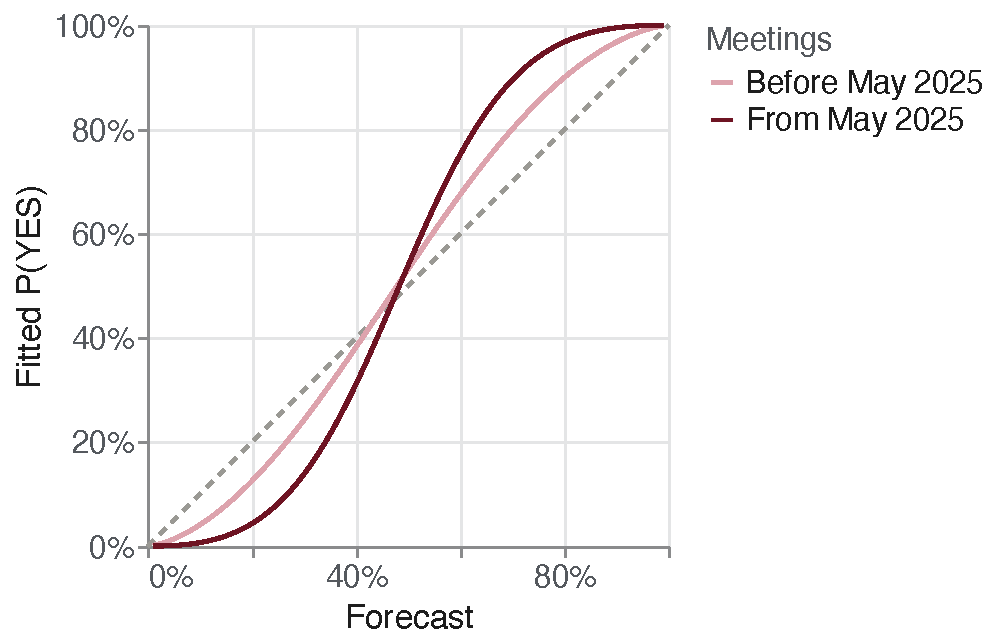
\includegraphics[height=5.6cm]{fitted_by_regime}
    \end{column}
    \begin{column}{0.36\textwidth}
      \vspace{10pt}
      \keyfig{1.49 $\rightarrow$ 2.35}{$\beta$ before vs.\ from May 2025}
      \keyfig{p = 0.19}{difference in $\beta$ (joint test p = 0.36, bootstrap)}
      {\footnotesize\color{sloangray}A large p-value means no detectable change, not no change. The regimes also differ in policy: mostly holds before, cuts after.\par}
    \end{column}
  \end{columns}
\end{frame}

\begin{frame}{Accuracy fades with horizon, and single surprises dominate}
  \framesubtitle{Log loss per meeting by days to meeting; labelled points are the largest misses}
  \source{02\_calibration\_kalshi.py}
  \centering
  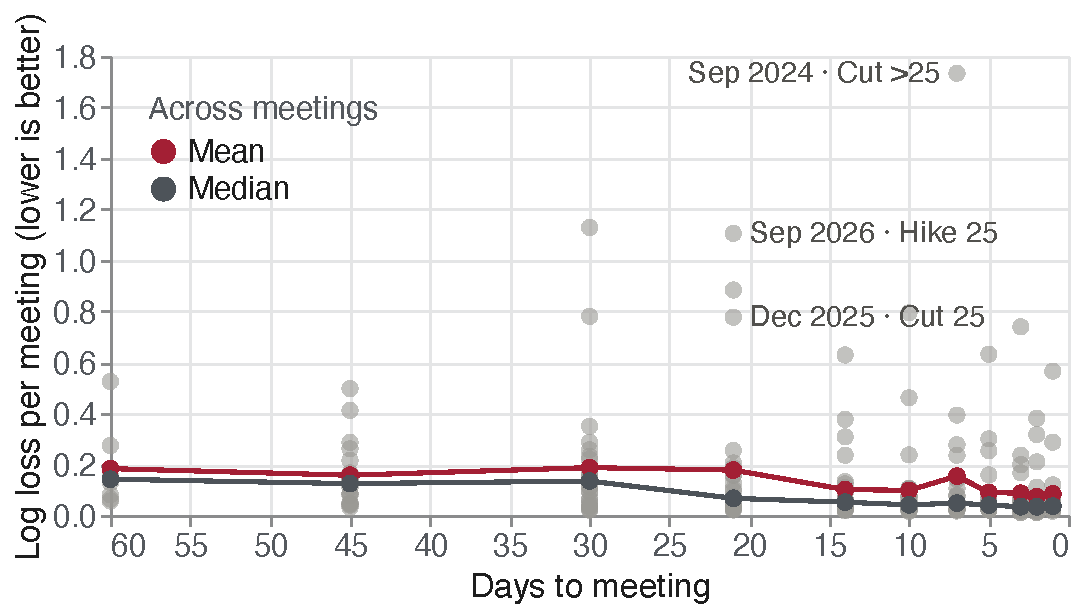
\includegraphics[height=5.2cm]{logloss_per_meeting}

  {\footnotesize\color{sloangray}Mean log score 0.07 at 1 day, 0.28 at 30 days; median at 1--21 days 0.05 vs.\ mean 0.14.\par}
\end{frame}

\begin{frame}{Minute-level reliability shows the same S-shape}
  \framesubtitle{Descriptive only: raw mid quotes every minute, 0--60 days, includes meeting day}
  \source{02\_calibration\_kalshi.py}
  \centering
  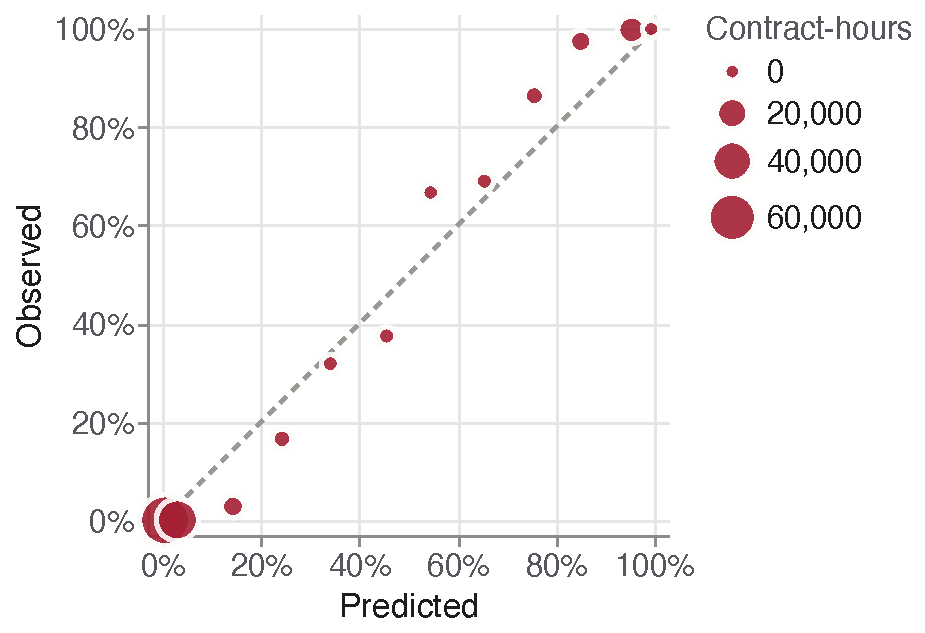
\includegraphics[height=5.6cm]{reliability_minute}
\end{frame}

\begin{frame}{Specification fixed before any significance test}
  \begin{columns}[T]
    \begin{column}{0.47\textwidth}
      \begin{itemize}\footnotesize
        \item Forecast: 16:00 ET bid--ask mid, $h \in \{1,2,3,5,7,10,14,21,30,45,60\}$ days before.
        \item Horizon groups: 1--21 days (main), 30, 45--60.
        \item Fed buckets normalized to sum to 1 (overround $\approx$ 1.5\%); raw as robustness.
        \item Tick-floor quotes (below 1\textcent, 0\textcent{} bid) excluded; included as robustness.
      \end{itemize}
    \end{column}
    \begin{column}{0.47\textwidth}
      \begin{itemize}\footnotesize
        \item Stale quotes kept and flagged; drop-stale as robustness. No spread filter.
        \item Scores per contract (log loss, calibration regression) and per meeting (log score, Brier).
        \item Minute-level results are descriptive only.
        \item Voided contracts and one untraded duplicate Fed event dropped.
      \end{itemize}
    \end{column}
  \end{columns}
  \vspace{10pt}
  {\footnotesize\color{sloangray}With about 28 meetings the test has low power, so the specification is fixed in advance.\par}
\end{frame}

\section{CPI \& payrolls}
\begin{frame}{CPI is under-confident, payrolls over-confident}
  \framesubtitle{1--21 days before the release; 18,049 forecasts, 203 releases; SEs clustered by release date}
  \source{03\_calibration\_macro.py}
  \begin{columns}[T]
    \begin{column}{0.5\textwidth}
      \centering
      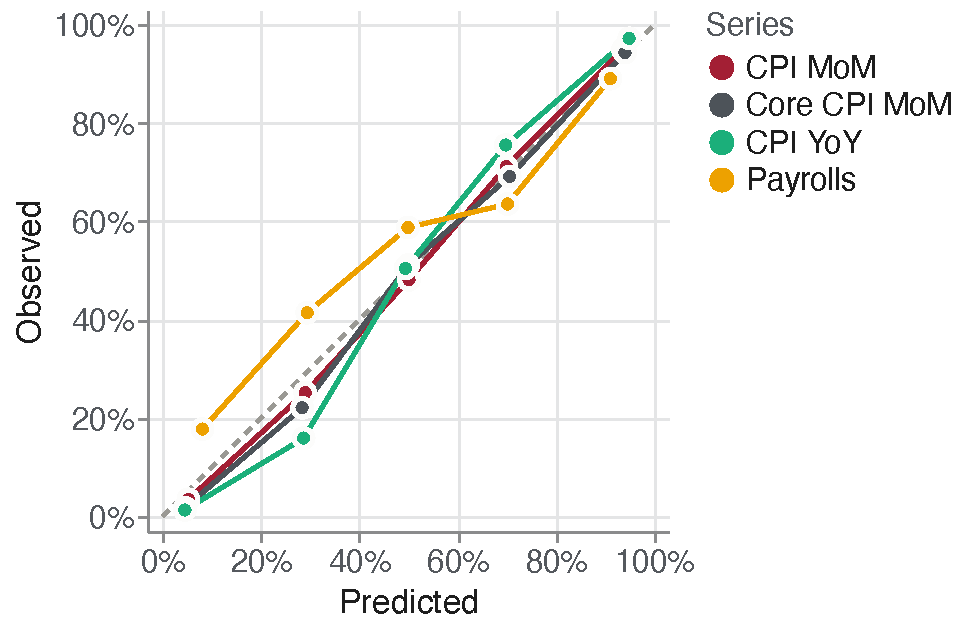
\includegraphics[height=5.1cm]{macro_by_series}
    \end{column}
    \begin{column}{0.46\textwidth}
      \centering\footnotesize
      \begin{tabular}{lrr}
        \toprule
        Series & $\beta$ (SE) & p($\beta$=1) \\
        \midrule
        CPI m/m & 1.20 (0.10) & 0.043 \\
        Core CPI m/m & 1.25 (0.11) & 0.025 \\
        CPI y/y & 1.40 (0.19) & 0.033 \\
        Payrolls & 0.75 (0.10) & 0.015 \\
        \midrule
        CPI pooled & 1.28 (0.10) & 0.005 \\
        All series & 1.11 (0.07) & 0.123 \\
        \bottomrule
      \end{tabular}
      \par\vspace{8pt}\raggedright
      {\footnotesize\color{sloangray}Reliability by series (left). Every $\alpha$ is insignificant. Ladder contracts are not exclusive, so prices are not normalized.\par}
    \end{column}
  \end{columns}
\end{frame}

\section{Futures}
\begin{frame}{How futures-implied probabilities are computed}
  \source{Literature/fed\_funds\_implied\_probabilities.pdf}
  \begin{itemize}\footnotesize
    \item FF$n$ settles on the average EFFR of month $n-1$, so the implied average for month $j$ is $\bar r_j = 100 - P_{j+1}$.
    \item A meeting on day $d$ of an $N$-day month splits it: $\bar r_j = \tfrac{d}{N} r_{\text{pre}} + \tfrac{N-d}{N} r_{\text{post}}$.
      \begin{itemize}\footnotesize
        \item Method A solves for $r_{\text{post}}$ and amplifies noise by $N/(N-d)$.
        \item Method B (preferred) takes $r_{\text{post}}$ from the next meeting-free month.
      \end{itemize}
    \item Meetings are chained; the start rate is the range midpoint plus a 10-day median EFFR spread.
    \item Expected move $x$ in 25bp steps: with $n = \lfloor x \rfloor$, $p = x - n$, the move is $n$ steps w.p.\ $1-p$ and $n+1$ steps w.p.\ $p$.
    \item Checks: all 2,909 (meeting, date) pairs sum to 1; Methods A and B differ by a median of 1.4bp.
  \end{itemize}
\end{frame}

\begin{frame}{One meeting up close: September 2024}
  \framesubtitle{Probability of a cut larger than 25bp; the Fed cut 50bp}
  \source{03\_fedfunds\_vs\_kalshi.py}
  \centering
  \begin{tikzpicture}
    \begin{axis}[sloan, width=12cm, height=5.5cm,
        xmin=-50, xmax=0.5, ymin=0, ymax=1, xlabel={Days before the meeting},
        ytick={0,0.25,0.5,0.75,1}, legend style={at={(0.36,0.98)}, anchor=north west}]
      \addplot[kalshiline, line width=1pt, no marks] table[x=t, y=mid] {data/sep24_kalshi_c50.dat};
      \addlegendentry{Kalshi (6-hourly mid)}
      \addplot[benchline, no marks, const plot] table[x=t, y=p_ff] {data/sep24_ff_c50.dat};
      \addlegendentry{Futures (daily)}
    \end{axis}
  \end{tikzpicture}
\end{frame}

\begin{frame}{Kalshi and futures agree closely near the meeting}
  \framesubtitle{Mean absolute gap in probability, hold and $\pm$25bp outcomes; 14,513 contract-days}
  \source{03\_fedfunds\_vs\_kalshi.py}
  \centering
  \begin{tikzpicture}
    \begin{axis}[sloan, width=11cm, height=5.3cm, ybar, sloanbars, bar width=16pt, ymin=0, ymax=0.13,
        xtick=data, xticklabels from table={data/ff_vs_kalshi_gap.dat}{horizon},
        xlabel={Days before the meeting}, ylabel={Mean abs.\ gap},
        yticklabel style={/pgf/number format/fixed, /pgf/number format/precision=2},
        nodes near coords, nodes near coords style={font=\tiny, color=ink,
          /pgf/number format/.cd, fixed, precision=3}]
      \addplot[fill=sloanred, draw=none] table[x=i, y=mad] {data/ff_vs_kalshi_gap.dat};
    \end{axis}
  \end{tikzpicture}

  {\footnotesize\color{sloangray}Correlation falls from 0.998 (1 day) to 0.928 (121+ days).\par}
\end{frame}

\begin{frame}{Reliability: futures vs.\ Kalshi}
  \framesubtitle{Hold and $\pm$25bp outcomes, 1--30 days pooled; bins from 0.3 to 0.6 hold 2--5 meetings}
  \source{03\_fedfunds\_vs\_kalshi.py}
  \centering
  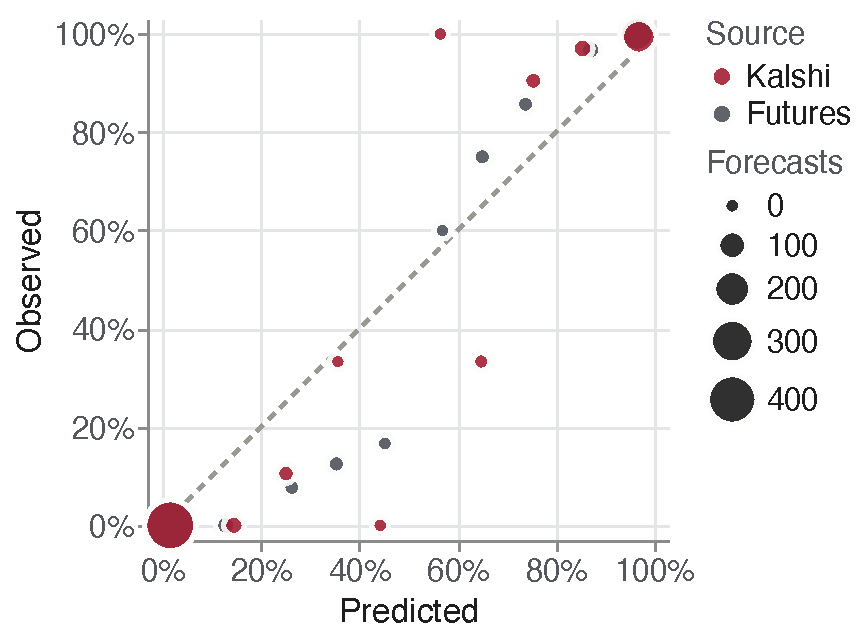
\includegraphics[height=5.6cm]{ff_vs_kalshi_reliab}
\end{frame}

\begin{frame}{Scores: Kalshi vs.\ futures by horizon}
  \source{03\_fedfunds\_vs\_kalshi.py}
  \centering\footnotesize
  \begin{tabular}{lrrrrrr}
    \toprule
    Days before & 1 & 7 & 21 & 30 & 45 & 60 \\
    \midrule
    Brier, futures & 0.0049 & 0.0198 & 0.0425 & 0.0459 & \textbf{0.0222} & \textbf{0.0532} \\
    Brier, Kalshi & \textbf{0.0044} & \textbf{0.0191} & \textbf{0.0383} & \textbf{0.0392} & 0.0310 & 0.0755 \\
    \midrule
    Log loss, futures & 0.035 & \textbf{0.081} & 0.148 & 0.170 & \textbf{0.113} & \textbf{0.192} \\
    Log loss, Kalshi & \textbf{0.030} & 0.084 & \textbf{0.138} & \textbf{0.153} & 0.142 & 0.253 \\
    \bottomrule
  \end{tabular}

  \vspace{10pt}
  {\color{sloangray}Bold: lower (better) score. 28 meetings at 1--21 days, 8 at 60 days. Probabilities clipped to [0.005, 0.995].\par}
\end{frame}

\section{Lead--lag}
\begin{frame}{Lead--lag: data and method}
  \source{04\_leadlag\_fedfunds\_kalshi.py}
  \begin{itemize}\footnotesize
    \item \textbf{Futures:} Bloomberg 1-minute bid/ask bars, 30 Mar -- 12 Oct 2026, contracts Mar--Dec 2026; expected move per minute with the daily method (A or B per meeting). Median spread 0.5bp.
    \item \textbf{Kalshi:} expected move $\sum_k q_k \cdot \text{move}_k$ from 1-minute bucket mids, rescaled to sum to 1, carried onto the CME minute grid.
    \item \textbf{Alignment:} Bloomberg bars are labelled by start minute, so they are shifted one minute to match Kalshi. Without it the futures appear to lead by exactly one minute.
    \item \textbf{Validation:} at 15:00 the minute series matches daily settlements: 135 days, correlation 0.998, median gap 0.27bp.
    \item \textbf{Tests} on 5-minute changes (95\% of futures and 92\% of Kalshi changes are zero): cross-correlations, Granger regressions with 6 lags clustered by session, and paths after the largest 0.1\% of 1-minute moves.
  \end{itemize}
\end{frame}

\begin{frame}{The two markets track the same expectations}
  \framesubtitle{Expected move at the 16 Sep 2026 meeting, every 15 minutes (CME hours)}
  \source{04\_leadlag\_fedfunds\_kalshi.py}
  \centering
  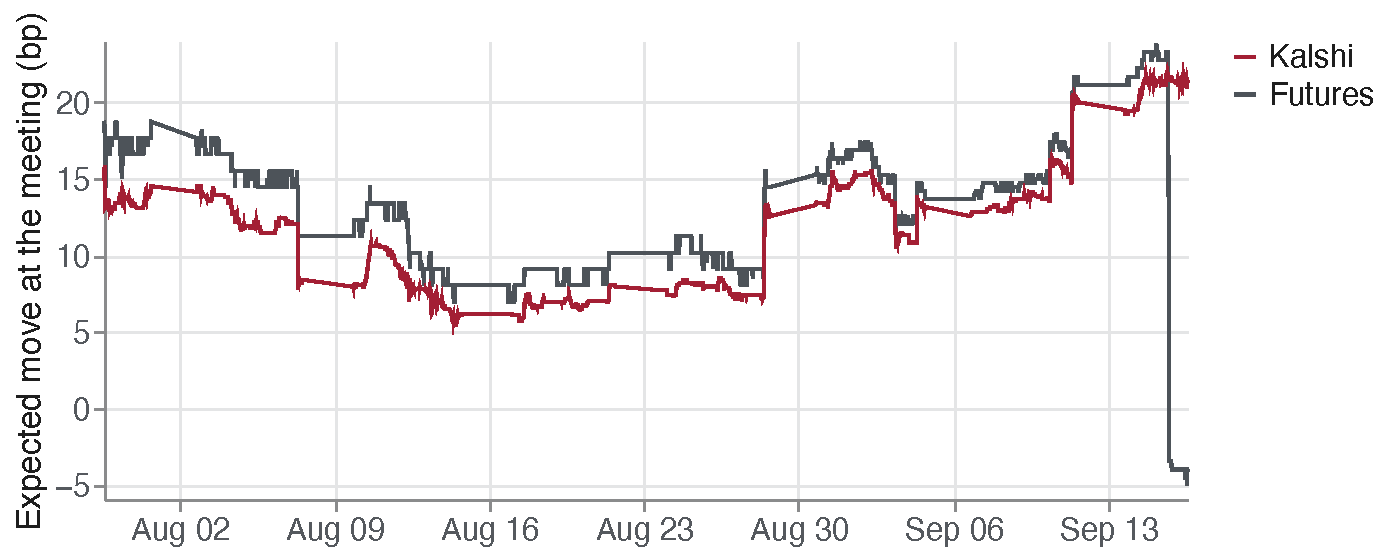
\includegraphics[width=0.92\linewidth]{leadlag_sep26_path}
\end{frame}

\begin{frame}{Granger tests: futures predict Kalshi, much less the reverse}
  \source{04\_leadlag\_fedfunds\_kalshi.py}
  \centering\footnotesize
  \begin{tabular}{lrrr}
    \toprule
    Question & Wald $\chi^2$ (6 df) & p-value & Sum of cross lags (SE) \\
    \midrule
    Do past futures moves predict Kalshi? & 30.30 & $<$0.001 & 0.133 (0.030) \\
    Do past Kalshi moves predict futures? & 12.02 & 0.062 & 0.279 (0.090) \\
    \bottomrule
  \end{tabular}

  \vspace{10pt}
  \raggedright
  {\footnotesize 37,632 five-minute changes, 140 sessions (all CME hours), 6 lags = 30 minutes, SEs clustered by session.\par
  \vspace{6pt}\color{sloangray}Caveats: about 140 days and five meetings; mostly-zero changes; different tick sizes (futures 0.25--0.5bp, Kalshi 0.25bp per cent); quotes, not trades.\par}
\end{frame}

\begin{frame}{After a large move, the other market follows only partly}
  \framesubtitle{Cumulative change divided by the size of the move, top 0.1\% of 1-minute moves}
  \source{04\_leadlag\_fedfunds\_kalshi.py}
  \centering
  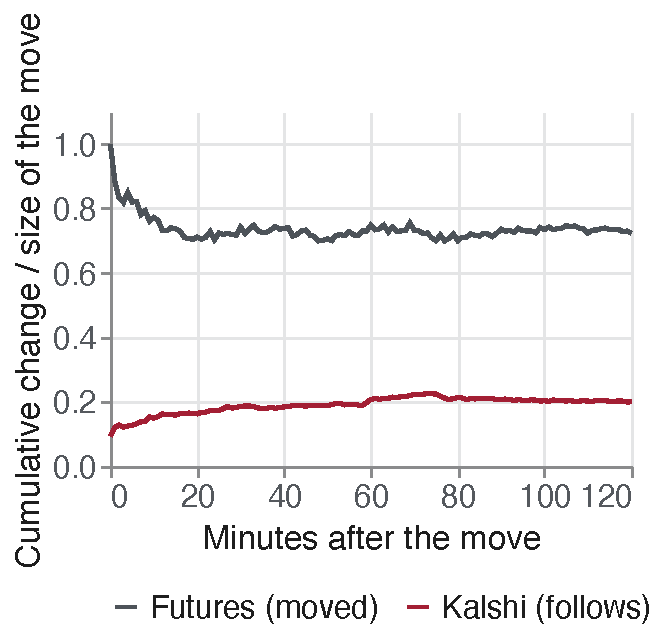
\includegraphics[height=4.9cm]{leadlag_after_futures}\hspace{0.6cm}
  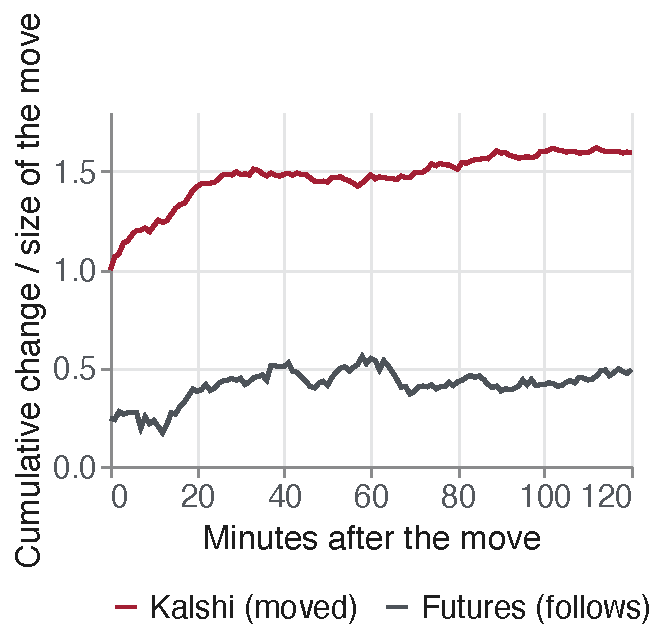
\includegraphics[height=4.9cm]{leadlag_after_kalshi}

  \vspace{4pt}
  {\footnotesize\color{sloangray}Futures moves (210, avg.\ 1.29bp): Kalshi follows 16\% within 15 minutes, 20\% within 2 hours. Kalshi moves (195, avg.\ 0.58bp): Kalshi builds to 160\% and futures follow 49\% within 2 hours.\par}
\end{frame}

\end{document}
